
\section{Taglio}
		Si vuole studiare quella sollecitazione caratterizzata da un certo carico lineare risultante $T_y$ alla faccia terminale della sezione.
	
		Una forza $T_y$ così applicata porta ad avere per equilibrio, sulla faccia iniziale, la presenza contemporanea di una $T_y$ uguale e opposta. 
	
		Tali forze così applicate però sono in equilibrio? A traslazione si, a rotazione no.
	
		Si vedrà così l'insorgenza di una coppia, di un momento $M_x$ sulla faccia iniziale della trave. \newline 
	
		Non esiste sforzo di taglio senza l'insorgenza di flessione secondaria. La sollecitazione di taglio è sempre accompagnata da una sollecitazione di momento flettente. 
	
\begin{figure}[H]
	\centering
	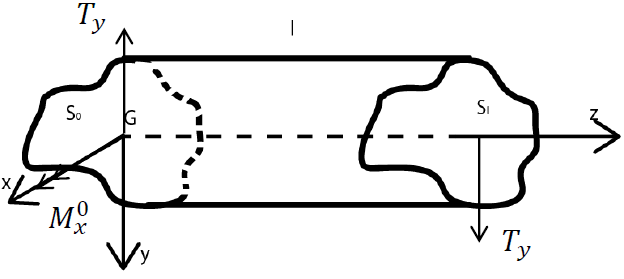
\includegraphics[width=0.5\linewidth]{immagini_6/screenshot001}
	\label{fig:screenshot001}
\end{figure}


		Un taglio è principale se viene applicato sulla direzione principale e porta a flessione retta; un taglio è deviato se non è applicato lungo una qualsivoglia direzione principale, si comporta come una composizione di tagli deviati e porterà a flessione deviata. \newline 
		
		Si studi l'equilibrio sulla faccia finale tramite il consolidato approccio alle tensioni: 
		\[ T_x = \int_A \tau_{zx}dA  = 0 \hspace{1cm}  T_y = \int_A \tau_{zy}dA  \hspace{1cm} N = \int_A\sigma_zdA = 0\]	
		Una qualunque distribuzione $\sigma_z$ che non sia banale genererebbe, seppur a risultante nulla in traslazione, un momento non nullo sulla faccia $S_l$, mentre invece si è imposto un momento flettente su tale faccia nullo, d'altronde per Cauchy, com'è che devono essere i vettori sulla faccia terminale per rispettare le condizioni al contorno? Uscenti dalla sezione finale, ma non essendo applicato alcuno sforzo normale, le uniche tensioni che applica $T_y$ sono delle $\tau_{zy}$.  \newline 
		
		Cosa risulta dall'equilibrio interno?
		\[
		\begin{cases}
			\begin{aligned}
				\frac{\partial \tau_{zx}}{\partial z} & =0 \\
				
				\frac{\partial \tau_{zy}}{\partial z} & =0 \\
				
				\frac{\partial \tau_{xz}}{\partial x} + \frac{\partial \tau_{yz}}{\partial y} + \frac{\partial\sigma_z}{\partial z} & =0 \\
			\end{aligned}
		\end{cases}
		\]
		Dalla $III$ equazione si vede che, se esistono delle $\tau_{zy}, \tau_{zx}$ la cui derivata è nulla, devono essere pari a \(\frac{\partial\sigma_z}{\partial z}\).
		
		Se si ipotizza una $\sigma_z$ costante lungo l'asse $z$ tale derivata è nulla e il problema sarebbe riconducibile al caso della flessione: con le stesse ipotesi ci si riconduce alle stesse soluzioni. 
		
		Ci si aspetta invece che $\sigma_z(z)\neq0$, variabile in $z$ perché, seppur in $S_l$ non ci sia momento, in $S_0$ esiste eccome, e cos'è che genera un momento flettente su quella faccia? Da cosa sono equilibrati gli $M_x$? Da delle tensioni normali $\sigma_z$!
		
		$\sigma_z$ esiste sulla faccia $S_0$ e non è vero che \(\frac{\partial\sigma_z}{\partial z} = 0\). \newpage
		
		Se si traccia il diagramma delle sollecitazioni:
		
		
\begin{figure}[H]
	\centering
	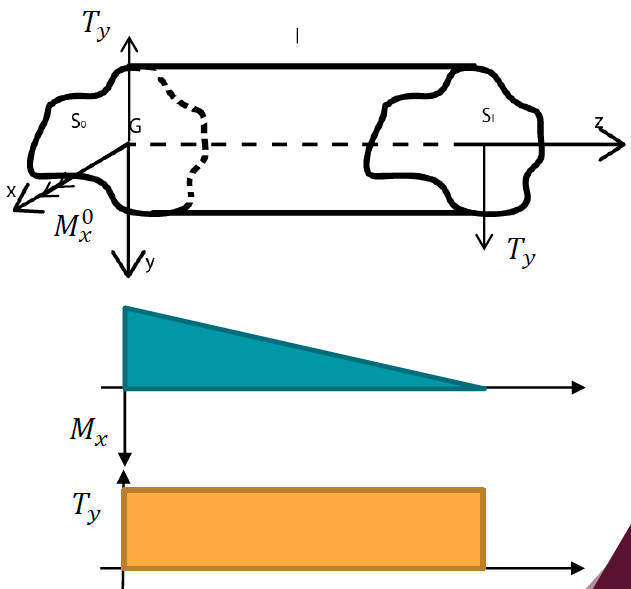
\includegraphics[width=0.5\linewidth]{immagini_6/screenshot002}
	\label{fig:screenshot002}
\end{figure}

		Si nota che a seguito dell'applicazione $T_y$ si avrà un taglio costante su tutta la trave, una sollecitazione di momento flettente che non è più costante lungo tutta la trave, al contrario delle flessione retta; e una sollecitazione flessione con un momento flettente che non è più costante lungo tutta la trave ma linearmente variabile, con che legge varia? Attraverso le equazioni indefinite di equilibrio so ricondurmi ad un andamento simile:
		\[M^0_x=-T_yL\]
		Dove il segno meno tiene conto che il momento applicato è in verso orario anziché antiorario. \newline 
		
		Per sezione generica a quota $z$: 
		\[M_x=-T_y(L-z) =T_y(z-L) \]
		Che verifica inoltre la condizione per cui, se $z=L$:
		\[M^L_x=0\]
		
		Se il momento flettente ORA varia con la quota $z$, le tensioni $\sigma_z$, avranno sì andamento simile a quello del momento flettente, ma variabile proprio lungo la $z$.
		
		D'altronde, una volta che con De Saint Venant so ricavarmi alla generica sezione quanto valgono le caratteristiche della sollecitazione non ci sarà più bisogno di risolvere ogni volta il problema, userò quel valori ottenuti per ricavare le tensioni: attraverso le caratteristiche della sollecitazione per quella sezione costruirò con DSV la distribuzione di tensione su quella sezione, anche a partire dai valori numerici di momento, taglio e sforzo.
		
		Per flessione retta valeva: 
		\[\sigma_z = \dfrac{M_x}{I_x}y = \dfrac{T_y(z-L)}{I_x}y\]
		E il diagramma a farfalla diminuirà d'intensità lungo le sezioni.

\begin{figure}[H]
	\centering
	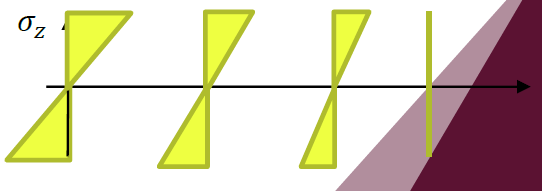
\includegraphics[width=0.5\linewidth]{immagini_6/screenshot003}
	\label{fig:screenshot003}
\end{figure}

		Si conferma così che la tensione normale non è solo dipendente da $y$ ma anche da $z$.\newline 
		
		Il risultato di uno sforzo di taglio applicato all'estremo della trave genera tensioni normali variabili in $z$ ed $y$ e tensioni tangenziali, per la valutazione di queste ultime sorgono non pochi problemi da affrontare. \newline 
		
		La risultante del taglio cambia l'entità del valore della tensione e la sua tipologia in base alla sua retta d'azione.
		
		Per i momenti era d'interesse il solo asse dei momenti che tutt'al più poteva essere baricentrico, con lo sforzo normale invece in dipendenza che l'asse di applicazione fosse baricentrico o meno, generava trazione o pressoflessione. 
		
		Il taglio genera una casistica simile a quella della pressoflessione, sebbene con sia più il baricentro il punto d'interesse: se si sta considerando come prima ipotesi un taglio $T_y$ su asse principale d'inerzia (se così non fosse basterebbe una composizione lungo tali assi), l'importante è che l'asse delle linee di forza passi per un punto specifico chiamato centro di taglio $C_t$, qualora la forza passasse per questo centro di taglio le azioni che si stabilirebbero sarebbero esclusivamente di taglio, un \textbf{taglio puro}, qualora invece questa forza non passasse per questo centro di taglio, oltre alla generazione di sforzi di taglio, normali e flessionali, genererebbe anche delle azioni tangenziali di torsione. \newline 
		
		 Quando $T_y$ passa per un punto $C_t$ non c'è torsione.
		 
		 Il che si traduce nel dire che  torsione e taglio sono ortogonali in energia: le sollecitazioni di taglio non compiono lavoro virtuale con un possibile campo di spostamenti (deformazioni) associato alla torsione. \newline
		 
		 Nella pratica si ottengono le seguenti equazioni per le coordinate di $C_t$:
		 \[  x_t = {1\over T_y} \int_A\omega \cdot \left(\vec{\nabla}\cdot\vec{\tau}_z\right) = -{1\over I_x}\int_A\omega\cdot ydA \hspace{1cm} y_t = -{1\over I_y}\int_A\omega\cdot xdA\]
		 Entrambe dipendenti dalla funzione ingobbamento. 
		 
		 Si sfrutti qualche proprietà di questa funzione, noto che laddove la sezione è simmetrica o doppio simmetrica $\omega$ ha andamento simmetrico doppio simmetrico, questo si traduce nel dire che - ai fini del centro di taglio - se esiste un asse  di simmetria $C_t$ giace su tale asse, se esistono due assi di simmetria $C_t$ giace su entrambi gli assi, e come fa un punto a giacere su due rette? Vuol dire che è intersezione di queste, e qual è l'intersezione di due assi di simmetria? Il baricentro. 
		 
		 Qualora il centro di taglio non appartenesse agli assi di simmetria si vedrebbe l'applicazione di uno sforzo di torsione pari esattamente alla forza di taglio per la distanza tra la retta d'azione della forza ed il $C_t$: un momento torcente uniforme che si applica su tutta la trave. \newline 
		 
		 Che tensioni tangenziali genera una forza di taglio così orientata? Siccome non si riesce a risolvere questo problema in forma chiusa si applicherà un approccio semplificato con ipotesi altamente stringenti, accurato per sezioni in parete sottile e tutte le possibili combinazioni di tratti sottili (H, C, T, doppia T \dots) con applicazioni privilegiate per sezioni compatte con massa e area prossime al baricentro. 
		 
		 L'approccio sarà tanto più errato quanto più la sezione si inspessisce diventando frastagliata e irregolare, per cui tanto più è larga la sezione della direzione ortogonale al taglio, tanto più tali ipotesi perderanno validità.\newpage
		 
		 \textbf{HP}: Supponiamo di avere una sezione generica e di eseguire una suddivisione con una corda $b$ dividendo l'area in $A'$ ed $A''$ definisco poi i vettori $\hat{m} \perp b; \hat{l} \parallel b$. 
		 
\begin{figure}[H]
	\centering
	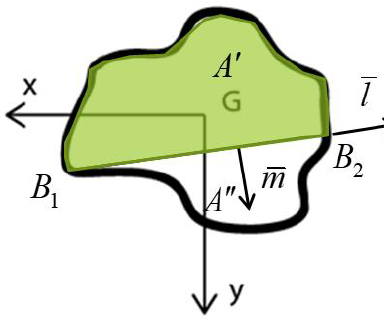
\includegraphics[width=0.5\linewidth]{immagini_6/screenshot004}
	\label{fig:screenshot004}
\end{figure}
		 
		 L'approssimazione sta nel dire che la distribuzione di $\tau$ lungo questa corda è una distribuzione di due componenti $\tau_{zm}\downarrow$ e $\tau_{zl}\rightarrow$ e dove più $\hat{m} \approx \hat{y}$ più la componente principale di tensione è la  $\tau_{zm}$ rispetto alla  $\tau_{zl}$. Inoltre più questi $\tau_{zm}$ sono principali, più la distribuzione reale è una distribuzione approssimabile ad un andamento continuo:
		 \[\tau_{zm} = {1\over b}\int_{B_1}^{B_2}\tau_{zm}ds\]
		 Più la sezione è sottile e più l'approssimazione è corretta: la distribuzione di tensioni sarà costante lungo l'ascissa curvilinea $l$ che si muove lungo la corda $b$. \newline 
		 
		 Si consideri una trave a sezione compatta e semplicemente connessa. Si ricordi poi come la $III$ equazione indefinita di equilibrio si possa scrivere: 
		 \[ \vec{\nabla}\cdot\vec{\tau}_z = -\dfrac{\partial \sigma_z}{\partial z} = -\dfrac{T_y}{I_x}y \]
		 Avere ora una divergenza non nulla implica avere delle linee di flusso non più chiuse ed avere linee di flusso aperte significa che lungo i percorsi - che ora avranno inizio e fine - si genereranno delle tensioni $\tau$ che varieranno lungo l'ascissa curvilinea. \newline 
		 
		\begin{itemize}
			 \item[$\rightarrow$] Integro direttamente $\tau_z$ che so lungo la corda essere costante:
		 \[ \int_{A'} \vec{\nabla}\cdot\vec{\tau}_z dA = \int_{\partial A'} \vec{\tau}_z \cdot \hat{m} ds + \underbrace{\int_{\partial A' -B_1B_ 2} \vec{\tau}_z \cdot \hat{m} ds}_\text{$0:\vec{\tau}_z\perp\hat{m}$ per le C.C.} = \int_{B_1}^{B_2} \vec{\tau}_z \cdot \hat{m} ds = \tau_{zm}b \]
		 \item[$\rightarrow$] Ma so che \( \vec{\nabla}\cdot\vec{\tau}_z = -\dfrac{T_y}{I_x}y\):
		 \[ \int_{A'} \vec{\nabla}\cdot\vec{\tau}_z dA = -\int_{A'}\dfrac{T_y}{I_x}ydA = -\dfrac{T_y}{I_x}S_x^{A'}\]
		 Allora necessariamente:
		 \[\tau_{zm}b = -\dfrac{T_y}{I_x}S_x^{A'} \]
		 \[ \tau_{zm} = -\dfrac{T_y}{I_x}\dfrac{S_x^{A'}}{b} \]
		 Tale formula prende il nome di \textbf{formula di Jourawski} ed è negativa se si prende in considerazione l'area superiore la corda. 
		\end{itemize} 
		 
		 Non si sono però verificate nè compatibilità, nè congruenza, ebbene, non li soddisfa entrambe, non è una soluzione esatta, approssima però correttamente lo stato tensionale. \newline 
		 
		 La stessa formula si può ricavare anche per equilibrio. 
		 
\begin{figure}[H]
	\centering
	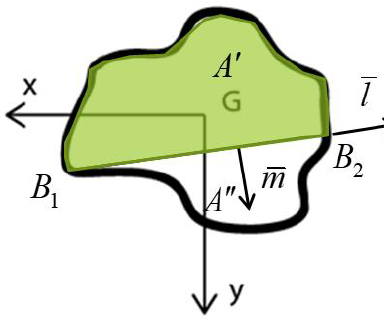
\includegraphics[width=0.3\linewidth]{immagini_6/screenshot004}
	\label{fig:screenshot004.2}
\end{figure}

		Che azioni interne si generano su una porzione della sezione? Applico lo studio all'area inferiore.

		La sollecitazione di taglio genera una $\tau_{zm}$, ma qual è il motivo per cui nascono queste tensioni sulla trave a seguito di una forza di taglio.
		
\begin{figure}[H]
	\centering
	\label{fig:screenshot005}
	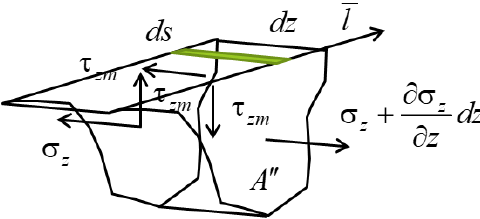
\includegraphics[width=0.5\linewidth]{immagini_6/screenshot005}
\end{figure}


		Separando le fibre del materiale, a seguito di una flessione, queste non occupano più la stessa posizione che occuperebbero se fossero state unite.
		
		Si scriva  l'equilibrio in direzione $z$ delle azioni sul volume di sezione $A''$:
		\[ -\int_{A''}\sigma_zdA + \int_{A''}\left(\sigma_z + \dfrac{\partial\sigma_z}{\partial z}dz\right)dA - \int_{B_1}^{B_2} \tau_{zm} \cdot dz ds = 0 \]
		\[ \int_{B_1}^{B_2} \tau_{zm} \cdot ds = \int_{A''}\dfrac{\partial\sigma_z}{\partial z} \]
		\[ \tau_{zm} = {1\over b} \int_{A''}\dfrac{T_y}{I_x}ydA = \dfrac{T_y}{I_x}\dfrac{S_x^{A''}}{b}\]
		Tale formula è perfettamente equivalente a quella poco sopra ricavata, dove la differenza risiede nel fatto che è positiva e si è presa in considerazione l'area inferiore la corda. \newline 
		
		D'altro canto per le proprietà booleane delle aree vale: 
		\[ S_x^{A} = S_x^{A'} + S_x^{A''} = 0 \Rightarrow S_x^{A'} = -S_x^{A''}\]
		Se si considera l'area contenente $\hat{m}$ si usa il $+$, se si considera l'area rispetto alla quale esce $\hat{m}$ si una il $-$.\newline 
		
		La relazione che abbiamo scritto dipende dal valore del taglio, dal valore del momento d'inerzia (e quindi dalla distribuzione d'area), dalla corda e dal momento statico, quello che non compare da nessuna parte è il punto d'applicazione del taglio $T_y$. \newline
		
		\textbf{NB}: ricorda che i momenti statici $ S_x^{A',A''} $ sono i momenti statici calcolati rispetto al baricentro dell'intera sezione. \newline
		
		Ora che con Jourawski si sono ricavate le $\tau_{zm}$ ci si chiede se le azioni che si sono trascurate, le $\tau_{zl}$, siano d'interesse o meno. 
		
		Sempre dalla $III$ equazione di equilibrio, se la l'operatore divergenza cambia variabili è lo stesso assicurata l'equivalenza delle derivate, per cui: 
		\[ \vec{\nabla}\cdot\vec{\tau}_z  -\dfrac{\partial \sigma_z}{\partial z} = 0\]
		\[ \dfrac{\partial \tau_{zl}}{\partial l} + \dfrac{\partial\tau_{zm}}{\partial m} + \dfrac{\partial\sigma_z}{\partial z} = 0\]
		Derivando per $l$ due volte ottengo: 
		\[ \dfrac{\partial^3 \tau_{zl}}{\partial l^3} + \dfrac{\partial^3\tau_{zm}}{\partial l^2\partial m} + \dfrac{\partial^3\sigma_z}{\partial l^2\partial z} = 0\]
		Ma derivando due volte rispetto ad $l$ il termine:
		\[\sigma_z =  \dfrac{T_y(z-L)}{I_x}y \rightarrow 0\]
		E dunque:
		\[ \dfrac{\partial^3 \tau_{zl}}{\partial l^3} = - \dfrac{\partial^3\tau_{zm}}{\partial l^2\partial m}\]
		L'ipotesi alla base del modello di Jourawski è che le $\tau_{zm}$ lungo la corda, sono costati, e cosa succede se derivo rispetto ad $l$ una grandezza costante rispetto ad $l$, che la sua derivata sarà nulla. 		
		\[ \dfrac{\partial^3 \tau_{zl}}{\partial l^3} = 0\]
		La tensione parallela alla corda allora potrà essere al più di secondo grado in $l$:
		\[ \tau_{zl} = al^2 + bl + c\]
		Con termini $a,b,c$ di volta in volta determinati tramite opportune condizioni al contorno. 
		
\subsection{ Taglio in sezioni compatte simmetriche}
		Come si traduce tutto ciò che è stato trattato fin'ora in termini applicativi? Su sezioni compatte e simmetriche la trattazione purtroppo produce qualche falla, ma quanto sono approssimati i risultati?
		
\begin{figure}[H]
	\centering
	\label{fig:screenshot006}
	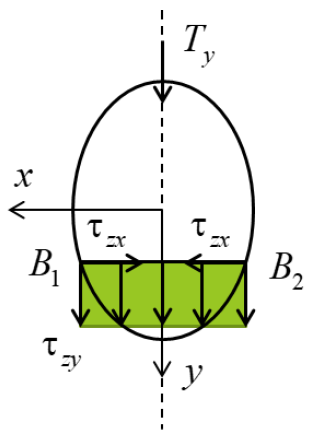
\includegraphics[width=0.2\linewidth]{immagini_6/screenshot006}
\end{figure}

		Essendo $y$ asse di simmetria e principale d'inerzia, se contiene $C_t$ e $G$, applicando una $T_y$ come in figura so che questa colpirà al $100\%$ il centro di taglio e sulla trave non si avrà nient'altro che un taglio puro: taglio con momento flettente. \newline 
		
		La tensione dipenderà così dalla quota $y$ piuttosto che da $x$, perché in questo caso è in funzione di $y$ che cambia il valore di $b$ ed $S_x$. 
		\[ \tau_{zm} = \tau_{zy} = \dfrac{T_y}{I_x}\dfrac{S_x^{A''}}{b}\]
		
		Come cambia $\tau$  in funzione che io mi trovi ai due apici della sezione? In questo tipo di sezione agli apici $b\rightarrow0$ e $S_x\rightarrow0$, ma a cosa si riconduceva il momento statico? Dalla definizione questo è l'area considerata per la distanza tra il baricentro dell'area considerata e l'asse rispetto al quale calcolo il momento statico stesso:
		\[S_x = A'' \cdot d(G_{A''}, x)\]
		Per entrambi gli apici, se si avesse soltanto $b\rightarrow0 \Rightarrow\tau\rightarrow\infty$ ma è assurdo perché $\tau$ è una grandezza fisica, si scopre così che all'apice superiore $S_x\rightarrow0$ molto più velocemente di $b$, in questo punto l'area sottesa dalla corda è tutta quella della sezione e $G_{A''}\equiv G$ ed ugualmente all'apice inferiore, molto più semplicemente è la stessa $A'' \rightarrow0$. \newline 
		
		Le tensioni così avranno un andamento che partirà dallo $0$ e ritornerà allo $0$, e non potevano fare altrimenti, d'altro canto delle tensioni tangenziali $\tau$ apicali non nulle avrebbero violato le condizioni al contorno di Cauchy. \newline 
		
		L'andamento delle tensioni tangenziali dipende da così da $S_x$ che ha un andamento quadratico/parabolico, per trovare il massimo di quest'andamento è sufficiente eseguire uno studio di funzione: 
		\[ {d\over dy}\tau_{zy} = {d\over dy}\left(\dfrac{T_y}{I_x}\dfrac{S_x^{A''}}{b}\right) = \dfrac{T_y}{I_x}\left( {1\over b}\dfrac{dS_x^{A''}}{dy} - \dfrac{S_x^{A''}}{b^2}\dfrac{db}{dy}\right) = 0\]
		Ma \( dS_x^{A''} = ybdy\) e così
		\[ \dfrac{T_y}{I_x}\left( {1\over b}\dfrac{dS_x^{A''}}{dy} - \dfrac{S_x^{A''}}{b^2}\dfrac{db}{dy}\right) = 0 \]
		Se e solo se è vero che:
		\[{1\over b}\dfrac{ybdy}{dy} = \dfrac{S_x^{A''}}{b^2}\dfrac{db}{dy}\]
		E dunque: 
		\[ y =  \dfrac{S_x^{A''}}{b^2}\dfrac{db}{dy}\]
		Viene fuori che la quota dove tale funzione è massima è la quota $y$ del baricentro, qualora, in corrispondenza di $G$, la corda $b$ abbia un valore massimo, o meglio qualora in corrispondenza di $G$ la derivata di $b$ rispetto ad $y$ sia nulla. 
		
		Se contemporaneamente alla quota baricentrica abbiamo anche una pendenza del fianco della sezione verticale allora quello sarà un punto di massimo dell'andamento del taglio. \newline 
		
		In questo caso oltre a notare che alla quota baricentrica la pendenza è verticale, si riporta anche l'andamento a farfalla delle $\sigma_z$. 
		
\begin{figure}[H]
	\centering
	\label{fig:screenshot007}
	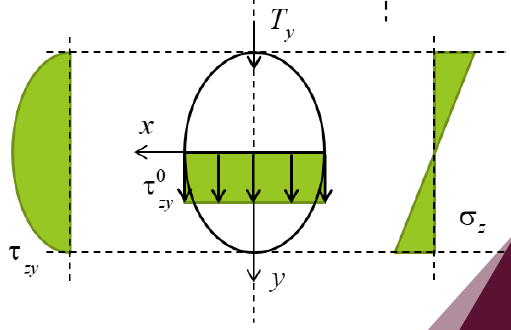
\includegraphics[width=0.45\linewidth]{immagini_6/screenshot007}
\end{figure}

		L'andamento delle tensioni $\tau_{yz}$ sulla corda generica non soddisfa però le condizioni al contorno, queste verificate solamente agli apici e agli estremi: ecco la prima forte approssimazione per sezione compatta. \newline 
		
		Per ripristinare le condizioni al contorno ho bisogno di una seconda componente di $\vec{\tau}$: dev'esserci anche un $\tau_{zx}$ tale che la combinazione lineare di $\tau_{xz}$ e $\tau_{zy}$ dia una tangenza al bordo della sezione la cui direzione determini un angolo $\gamma$. \newline
		
		La $III$ equazione di equilibrio, derivata una seconda volta rispetto ad $x$:
		\[\frac{\partial^2 \tau_{xz}}{\partial^2 x} + \cancel{\frac{\partial^2 \tau_{yz}(y)}{\partial x\partial y}} + \cancel{\frac{\partial\sigma_z(y,z)}{\partial x\partial z}}  =0\]
		\[ \frac{\partial^2 \tau_{xz}}{\partial^2 x} = 0\]
		Mi aspetto così una tensione $\tau_{xz}$ che varia al più secondo una legge lineare del tipo: 
		\[\tau_{xz} = \alpha x + \beta = 0\]
		Per risolvere il problema proposto ho bisogno di due condizioni al contorno , ricavabili queste dalle condizioni estremali su $B_1$ e $ B_2 $. 
		
\begin{figure}[H]
	\centering
	\label{fig:screenshot008.1}
	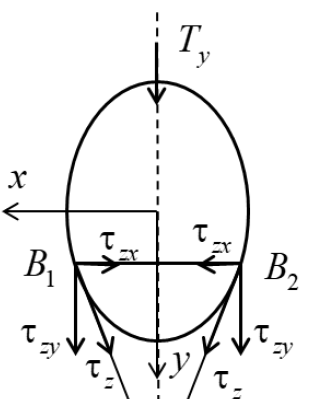
\includegraphics[width=0.2\linewidth]{immagini_6/screenshot008.1}
\end{figure}
		
		In $B_1$ $ \tau_{xz} $ è quella componente orizzontale tale che, combinata con la componente di Jourawski $ \tau_{yz} $, rende il vettore somma $\tau$ inclinato tangenzialmente al bordo, formando $\gamma$ con la verticale:
		\[ \begin{aligned}
			\tau_{xz}\left({b\over 2}, y\right) & = \tau_{yz}(y)\cdot \tan\gamma \\
			\tau_{xz}\left({-b\over 2}, y\right) & = -\tau_{yz}(y)\cdot \tan\gamma
		\end{aligned}\]
	 	\[ \tau_{xz} = -{2\over b}x\tau_{yz}\tan\gamma\]
	 	Nascono così queste azioni ortogonali all'asse $y$ con andamento a farfalla con massimo alle estremità e nullo sull'asse. 
	 	
\begin{figure}[H]
	\centering
	\label{fig:screenshot008.2}
	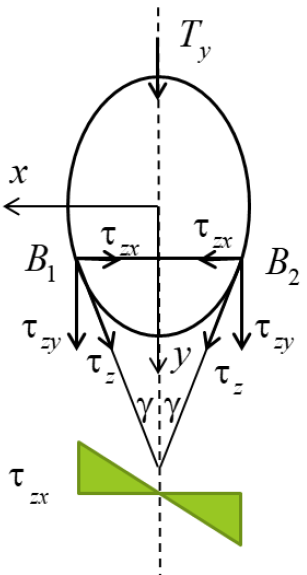
\includegraphics[width=0.15\linewidth]{immagini_6/screenshot008.2}
\end{figure}

		Chiudiamo la trattazione: quali sono le deformazioni associate alle azioni di taglio? Sicuramente si avranno degli scorrimenti angolari tra le facce che comporteranno certo abbassamento $d\eta$ al quale si aggiungerà un'inflessione dovuta al momento flettente $M_x$, che a meno che non sia un $M_x(z)$ la si sa già trattare: è ricavabile separatamente, sarebbe il contributo di abbassamento all'estremità di una mensola incastrata \(\dfrac{Ml}{EI}\) incontrato in \textit{meccanica dei solidi}, la rotazione dovuta alla flessione sarà così variabile lungo $ z $ in funzione del valore del momento flettente:
		\[ d\varphi = \dfrac{M_x}{EI_x}dz\]
		Il taglio applicato provoca anche un abbassamento dovuto allo slittamento di due facce della porzione di trave, pari ad una rotazione angolare per una lunghezza $dz$:
		\[d\eta = \Psi dz = \chi_y \dfrac{T_y}{GA}dz\]
		{\footnotesize (da meccanica dei solidi, parte 8 pag. 9)}\newline
		La rotazione angolare può essere valutata attraverso l'applicazione del principio dei lavori virtuali:
		\[ \Psi = \dfrac{T_y}{GA}\dfrac{A}{I_x^2}\int_{y_1}^{y_2}\dfrac{S_x^2}{b}\left(1 + {1\over 3}\tan^2\gamma\right)dy = \chi_y \dfrac{T_y}{GA} \] 
		Il fattore $\chi_y$ è chiamato fattore di taglio. \newline 
		
		\underline{In realtà} l'abbassamento alle estremità è dovuto all'inflessione della trave + un contributo dovuto al taglio, questo dovuto al fatto che le sezioni tra loro, a seguito dell'azione di taglio scorrono di una certa quantità l'una rispetto all'altra; l'ipotesi di Timoshenko e Bernoulli stanno a dire che questo scorrimento è o del tutto trascurabile, o da considerare, o da considerare così tanto che le sezioni oltre a scorrere, si ingobbano. \newline
		
		Oltre ad esserci scorrimento c'è anche una distorsione della sezione la quale si ingobbirà a causa del taglio.
		
		La sezione retta scorre, ma non subisce una distorsione angolare
		costante, poiché le tensioni tangenziali non lo sono. Negli estremi
		infatti le tensioni sono nulle, per cui l’angolo resta retto, causando
		un ingobbamento. 
		
\begin{figure}[H]
	\centering
	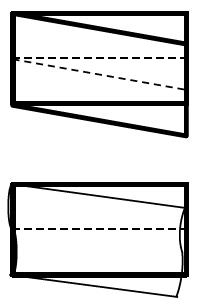
\includegraphics[width=0.15\linewidth]{immagini_6/screenshot008}
	\label{fig:screenshot008}
\end{figure}

		
		Naturalmente tutto ciò si valuterà laddove serva, in dipendenza che la trave sia snella non-snella o tozza, si valuteranno abbassamento e ingobbamento. 




%		\subsubsection{Sezione circolare}
%%\includepdf[pages={14}]{06_fcm_2022}
%
%\begin{figure}[H]
%	\includegraphics[scale=0.75,page=13]{06_fcm_2022}
%\end{figure}
%
%		Dov'è minimo l'andamento? Dov'è massimo? Dov'è zero? Sapendo che la sezione è compatta con $T_y$ in quella direzione, l'andamento sarà nullo alle estremità e massimo al baricentro, inoltre, sapendo che se in corrispondenza del baricentro \({db\over dy}=0\), quello sarà un punto di massimo, a maggior ragione se la derivata è nulla a causa della tangenza verticale. \newline 
%		
%		Dov'è massima la $\tau$ di taglio? Sul baricentro. 
%		
%		In quale sezione della trave? Il taglio lungo la trave è costante, ma se $\tau$ dipende esclusivamente da $T$ e dalla sezione e la sezione è costante per DSV, se $T$ è uguale per ogni ascissa curvilinea allora mi aspetto un massimo uguale ovunque rispetto a $z$ per ogni sezione; rispetto ad $y$ sarà invece massimo dove è $y$ ad essere massima e rispetto ad $x$ non importa perché alla fine punti alla stessa quota $y$ hanno tutti lo stesso valore. \newline 
%		
%		Ci si ricordi però che nasce anche un momento flettente. Nel momento in cui si effettueranno le verifiche oltre a preoccuparsi del taglio, sarà importante anche la quota di momento flettente, ma ancor di più la loro composizione: dove si sommano i loro effetti? Qual è il punto più sollecitato? 
%		
%		La verifica si fa come sempre confrontando una $\sigma$ con una $\sigma_a$ ammissibile, dove la $\sigma$ sarà la massima tra tutti i punti da valutare. 
%		
%		In questo caso, ad esempio, dove sarà? 
%		
%		Il momento flettente sarà massimo secondo il diagramma:
%		
%\begin{figure}[H]
%	\centering
%	\begin{tikzpicture}
%	\draw[thick] (0,0) -- (5,0);
%	\draw[pattern = vertical lines] (0,0) -- (0,2) -- (5,0) -- (0,0);
%\end{tikzpicture}
%\end{figure}
%
%		Mentre lo sforzo $\sigma_z$ sarà massimo lontano dall'asse, secondo questo diagramma:
%		
%\begin{figure}[H]
%	\centering
%	\begin{tikzpicture}
%		\draw[thick] (0,-1) -- (3,-1);
%		\draw[pattern = horizontal lines] (1,1) -- (3,1) -- (1,-1) --(1,1);
%		\draw[pattern = horizontal lines] (1,-1)-- (0,-2) -- (1,-2) -- (1,-1);
%	\end{tikzpicture}
%\end{figure}
%
%		Tutti i punti sollecitati a taglio sono sul $C_t\equiv G$, mentre quelli  a flessione sono quelli estremali, li valuto separatamente? 
%		
%		D'altronde dove è massimo uno è nullo l'altro e viceversa. \newline 
%		
%\subsection{ Taglio in sezioni sottili aperte  }
%
%\begin{figure}[H]
%\includegraphics[scale=0.75,page=14]{06_fcm_2022}
%\end{figure}
%
%
%		Sezione sottile, ovunque a pendenza costante \({\partial b\over \partial y} = 0\), l'asse di simmetria lungo il quale si va ad applicare il taglio è $y$ come in figura, in questo modo incontro sicuramente $G\equiv C_t$ e il taglio è puro. \newline		
%
%		Dove $y$ è la dimensione di $A'' $ mentre \( {h\over2} - y \over2\) è la distanza tra il baricentro di $A''$ e l'asse $x$ rispetto al quale si sta calcolando il momento statico. 
%		
%		L'asse baricentrico a pendenza verticale mi assicura che per il baricentro passerà il massimo della distribuzione di tensione. 
%		
%		La pendenza verticale inoltre implica che $\gamma=0$ ed esiste soltanto il contributo $\tau_{zy}$, esistono solo azioni tangenziali in direzione $y$, direzione del lato lungo della sezione.  
%		
%		Perché è così interessante la sezione sottile? Perché può essere combinata in più sezioni.  \newline 
%		
%\subsection{Taglio in sezioni sottili a doppia T}
%		La sezione a doppia T ha sicuramente due assi di simmetrica e il baricentro si troverà così come in figura. \newline 
%		
%		Le due propaggini superiore e inferiore si chiamano \textbf{ali}, mentre la sezione che collega le due ali si chiama \textbf{anima} centrale. \newline 
%		
%		Con una $T_y$ applicata come in figura lo sforzo sarà di taglio puro.
%		
%\begin{figure}[H]
%	\centering
%	\label{fig:screenshot009}
%	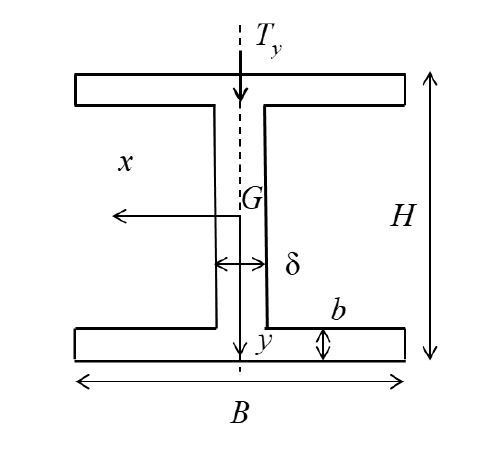
\includegraphics[width=0.3\linewidth]{immagini_6/screenshot009}
%\end{figure}
%
%		È una sezione che resiste ad alta flessione specifica, e com'è possibile generare una flessione? Con uno sforzo di taglio. \newline 
%		
%		Laddove la sezione risulti piccola, l'ipotesi di Jourawski è che tutto vada a collassare sulla linea media. 
%		
%		Si ragiona così lungo una linea media che passa per il centro, permettendo ciò di calcolare anche più agilmente i contributi $S_i, I_i$, perché si possono considerare i soli rettangoli componenti la sezione senza ripetizione o ridondanza di "elementini".\newline 
%		
%		Iniziamo a lavorare con Jourawski, mettiamoci su di una corda che taglia perpendicolarmente la linea media.
%		
%\begin{figure}[H]
%	\centering
%	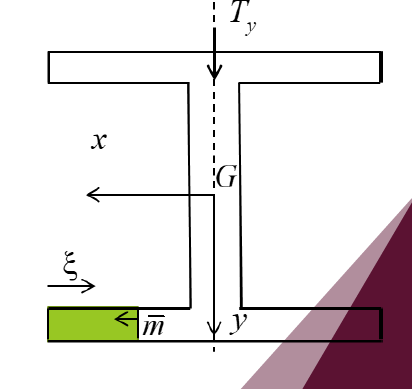
\includegraphics[width=0.3\linewidth]{immagini_6/screenshot010}
%	\label{fig:screenshot010}
%\end{figure}
%
%
%		Il momento d'inerzia dell'intera sezione è: 
%		\[ I_x = \dfrac{\delta H^3}{12} + 2\left[\dfrac{Bb^3}{12}  +Bb{H\over2}^2   \right]\]
%		ricordi che il primo termine è quello che passa per l'asse $x$ e il successivo moltiplicato per 2 è il termine lontano dall'asse delle due ali? Ricordi che un momento d'inerzia calcolato per una superficie lontana dall'asse vale  \(A\cdot D^2\)? \newline 
%		
%		Il momento statico dell'area considerata vale: 
%		\[S_x^{A''}= A'' \cdot d_xG'' + b\xi {H\over2}\]
%		Considerando sempre la struttura coincidente sulla linea media (quindi senza portarsi dietro gli elementini ($b/2$). \newline 
%		
%		\[ \tau_{zm(zx)} = \dfrac{T_y}{I_x}\dfrac{S_x^{A''}}{b} = \dfrac{T_y}{I_x} {H\over2}\xi \]
%		
%		L'andamento della tensione parte da $0$ e cresce linearmente con $\xi$, il risultato è positivo e dunque segue in direzione in versore $\hat{m}$. 
%		
%		Per simmetria applico la stessa risoluzione alla mezzala opposta. 
%		
%
%\begin{figure}[H]
%\includegraphics[scale=0.75,page=16]{06_fcm_2022}
%\end{figure}
%
%
%		Si salga adesso verso l'anima centrale, ora $ S_x^{A''} $ è data dal contributo intero dell'ala + il contributo del rettangolino $Y$ variabile questo con la quota $y$. \newline
%
%		Il momento statico sarà dato dall'area per la distanza dai baricentri, e per le due figure può essere composto: 
%		\[S_x^{A''}= A'' \cdot d_xG'' = Bb{H\over2} + \delta\left({H\over2} -y \right)\left({{H\over2} - y \over2} + y\right) = Bb{H\over2} + {\delta\over2}\left({H^2\over4}-y^2\right)\]
%		Il risultato? Una $\tau_{zm}$ funzione di secondo grado. Dove sarà il massimo? La quota baricentrica ha una corda che garantisce \({\partial b\over \partial y} = 0\), quindi si avrà alla quota baricentrica. 
%		\[ \tau_{zm(zy)}= \dfrac{T_y}{I_x}\dfrac{S_x^{A''}}{b} = \dfrac{T_y}{I_x\delta}\left[    \dfrac{bBH}{2} + {\delta\over2}\left({H^2\over4}-y^2\right) \right] \]
%
%		Per l'ala superiore, varranno le stesse considerazioni ma prese con verso opposto. 		
%
%		Tanto più è piccola la sezione, tanto più la situazione reale riflette quella qui riportata.  
%		
%		In analogia idrodinamica, la somma dei flussi entranti da sinistra e da destra, sarà uguale al flusso nell'anima:
%		\[2\tau_{zx} = \tau_{zy}\delta\] 
%		
%\subsection{Taglio in sezioni sottili a C}
%
%\begin{figure}[H]
%\includegraphics[scale=0.75,page=17]{06_fcm_2022}
%\end{figure}
%
%\begin{figure}[H]
%\includegraphics[scale=0.75,page=18]{06_fcm_2022}
%\end{figure}
%
%
%\subsection{Taglio in sezioni sottili chiuse}
%		Nel caso di sezioni chiuse la soluzione con Jourawski si può applicare solo in presenza di assi di simmetria, in assenza di simmetria Jourawski non basta, perché al suo interno comparirebbero due incognite, una $\tau$ da un lato e da un altro indipendenti tra loro, dovrei aggiungere le condizioni di compatibilità ma questo mi comporterebbe un aggravio della matematica. \newline
%		
%		Con simmetria è possibile ricavare Jourawski esattamente come visto fin'ora, è come integrare un'ala superiore della doppia T.  
%		
%\begin{figure}[H]
%	\centering
%	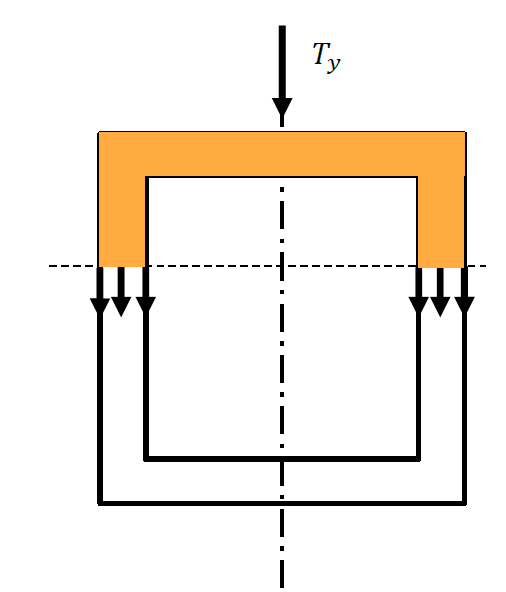
\includegraphics[width=0.3\linewidth]{immagini_6/screenshot011}
%	\label{fig:screenshot011}
%\end{figure}
%		
%		
%		Sfruttando la simmetria parto dall'asse della mezzala superiore e mi muovo ad esempio verso destra descrivendo la sezione d'interesse. 
%		
%		Ricordarsi che nelle sezioni laterali la larghezza della corda è doppi, perché sto prendendo due volte lo spessore. 
%		
%		Ci si riconduce sempre ad un andamento quadratico o lineare.
%        \[ \begin{matrix}
%        	S_x^{A'}= -2b\xi{H\over 2} &
%        		\tau_{zm(zx)} = \dfrac{T_y}{I_x}{H\over2}\xi \\
%        		S_x^{A''}= -Bb{H\over 2} - 2\delta\xi\left({H\over 2} - {\delta\over2}\right) &
%        		\tau_{zm(zy)}=  \dfrac{T_y}{I_x}\dfrac{HB}{4} + \dfrac{T_y}{I_x}\xi \left({H\over 2} - {\delta\over2}\right)
%        \end{matrix} \]
%    	In completa analogia idrodinamica, se un flusso entra dall'alto, nei punti in cui $\tau=0$, questo si divide, discende e si ricongiunge in basso. 
%    	\begin{figure}[H]
%    		\centering
%    		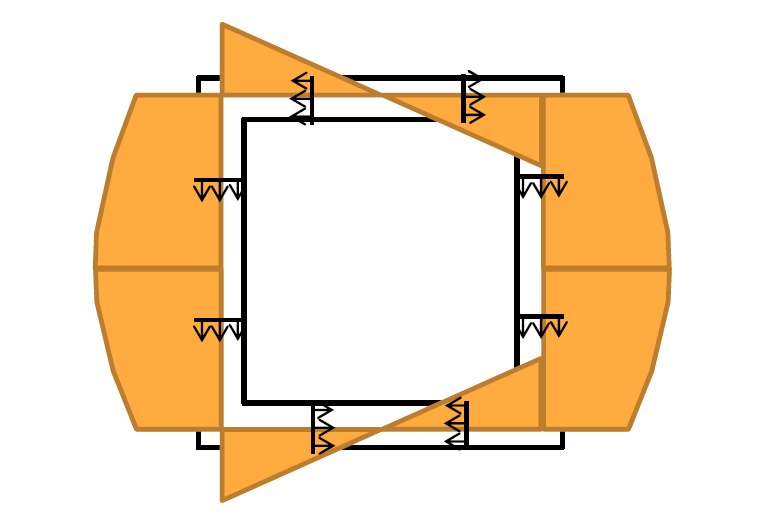
\includegraphics[width=0.5\linewidth]{immagini_6/screenshot012}
%    		\label{fig:screenshot012}
%    	\end{figure}
%    	 
%\subsection{Determinazione del centro di taglio}
%    	Sarà approfonditamente argomento di esercitazione. \newline 
%    	
%    	Se c'è un asse di simmetrica allo ra quello conterrà il $C_t$, se ci sono due assi di simmetria entrambi conterraneo il centro di taglio che si troverà a coincidere col baricentro.
%    	
%    	Generalmente si può dire che se ci sono due o più tratti di rettangoli e tutti questi concorrono in un unico punto senza fare percorsi multipli (sezioni a
%    	T,L,V,K,X…), allora quello sarà il centro di taglio. \newline 
%    	
%    	Dal punti di vista pratico il $C_t$ non è altro che un punto di equilibrio tra le azioni esterne ed interne: dato il momento risultante dal carico $T$ applicato nel $C_t$ rispetto ad un polo qualunque $P^*$, allora \( \int\tau_{taglio}\) dovrà dare lo stesso momento. \newline 
%    	
%    	Se ci si mette su $P^*$ e si guarda l'azione del momento esercitata da $T_y$ questa pari a \(T_y\cdot x_t\). 
%    	
%    	Ora, è iù che noto come le azioni esterne debbano stare in equilibrio con le azioni interne, se si integrano perciò le $\tau$ che seguono le facce, queste daranno tre contributi di forza nelle seguenti direzioni $\leftarrow, \downarrow, \rightarrow$: il momento risultante di questa forza rispetto al polo scelto dovrà così dare esattamente \(T_y\cdot x_t\), è in questo modo che si potrà trovare il centro di taglio. 
%    	
%\begin{figure}[H]
%	\centering
%	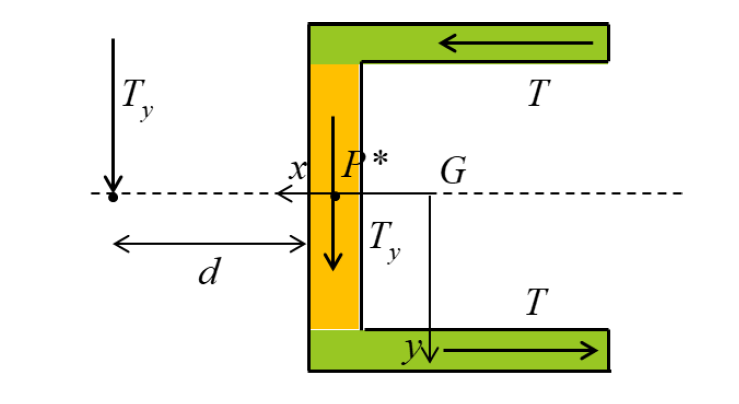
\includegraphics[width=0.3\linewidth]{immagini_6/screenshot013}
%	\label{fig:screenshot013}
%\end{figure}
%
%    	
%    	\[ \begin{aligned}
%    		T_x & = \int_{A^*}\tau_{xz}dA = \int_{0}^{B}\tau_{xz}bd\xi =\int_{0}^{B}\dfrac{T_yHB\xi}{2I_x}d\xi = \dfrac{T_yHB^2}{4I_x} \\
%    		T_y & = \int_{A^**}\tau_{xz}dA
%    	\end{aligned} \]
%    	\[ TH = T_yd \Rightarrow d = {TH\over T_y} = \dfrac{H^2bB^2}{4I_x}\]
%		
		\paragraph{Osservazioni finali}
		\begin{multicols}{2}
			\begin{itemize}\compresslist
			\item Le tensioni tangenziali sono le medesime in ogni sezione della trave e seguono la direzione della linea media
			alla quale sono parallele;
			\item Verso
			e intensità sono dettate dalla formula di Jourawsky, con direzione dipendente dalla linea media, segue la linea media;
			\item Il
			flusso delle tensioni tangenziali varia ed è continuo lungo la linea media.
			
			Il prodotto $\tau\delta$ che per torsione a sezione chiusa era costante, ORA NON È PIÙ COSTANTE, tant'è che è $0$ alle estremità e massimo alla quota baricentrica;
			\item Le
			tensioni tangenziali sono massime in corrispondenza dell’asse neutro di tensione;
			\item A seguito della \( \vec{\nabla}\cdot\vec{\tau}\ne0\) le
			linee di flusso sono curve aperte alle cui estremità c'è flusso nullo e dunque tensione nulla;
			\item Se i fianchi sono rettilinei a maggior ragione varrà \( \partial b\over\partial y = 0\) e $\tau$ sarà massima sulla quota baricentrica;
			\item La trattazione non si modifica se l’asse principale y non è di simmetria.
		\end{itemize}
		\end{multicols}
		
